\documentclass[12pt, a4paper]{article}  
\usepackage{etex}
\usepackage{amsmath,amsfonts,amssymb,amsthm,mathtools} 
\usepackage{fontspec}         
\setmainfont{Arial}   
\defaultfontfeatures{Mapping=tex-text}
\newfontfamily{\cyrillicfonttt}{Arial}
\newfontfamily{\cyrillicfont}{Arial}
\newfontfamily{\cyrillicfontsf}{Arial}
\usepackage{unicode-math}     % пакет для установки математического шрифта
\setmathfont{Asana Math}      % шрифт для математики

\usepackage{polyglossia}      % Пакет, который позволяет подгружать русские буквы
\setdefaultlanguage{russian}  % Основной язык документа
\setotherlanguage{english}    % Второстепенный язык документа


%%%%%%%%%% Работа с картинками %%%%%%%%%
\usepackage{graphicx}                  % Для вставки рисунков
\usepackage{graphics} 
\graphicspath{{images/}{pictures/}}    % можно указать папки с картинками
\usepackage{wrapfig}                   % Обтекание рисунков и таблиц текстом
\usepackage{subfigure}                 % для создания нескольких рисунков внутри одного


%%%%%%%%%% Работа с таблицами %%%%%%%%%%
\usepackage{tabularx}            % новые типы колонок
\usepackage{tabulary}            % и ещё новые типы колонок
\usepackage{array}               % Дополнительная работа с таблицами
\usepackage{longtable}           % Длинные таблицы
\usepackage{multirow}            % Слияние строк в таблице
\usepackage{float}               % возможность позиционировать объекты в нужном месте 
\usepackage{booktabs}            % таблицы как в книгах!  
\renewcommand{\arraystretch}{1.3} % больше расстояние между строками

\author{Маликова Ольга} 
\title{Домашнее задание 2}
\date{\today}

\begin{document} 

\maketitle

\section{Упражнение 1}

\begin{figure}[h!]
\begin{minipage}[h!]{0.3\linewidth} 
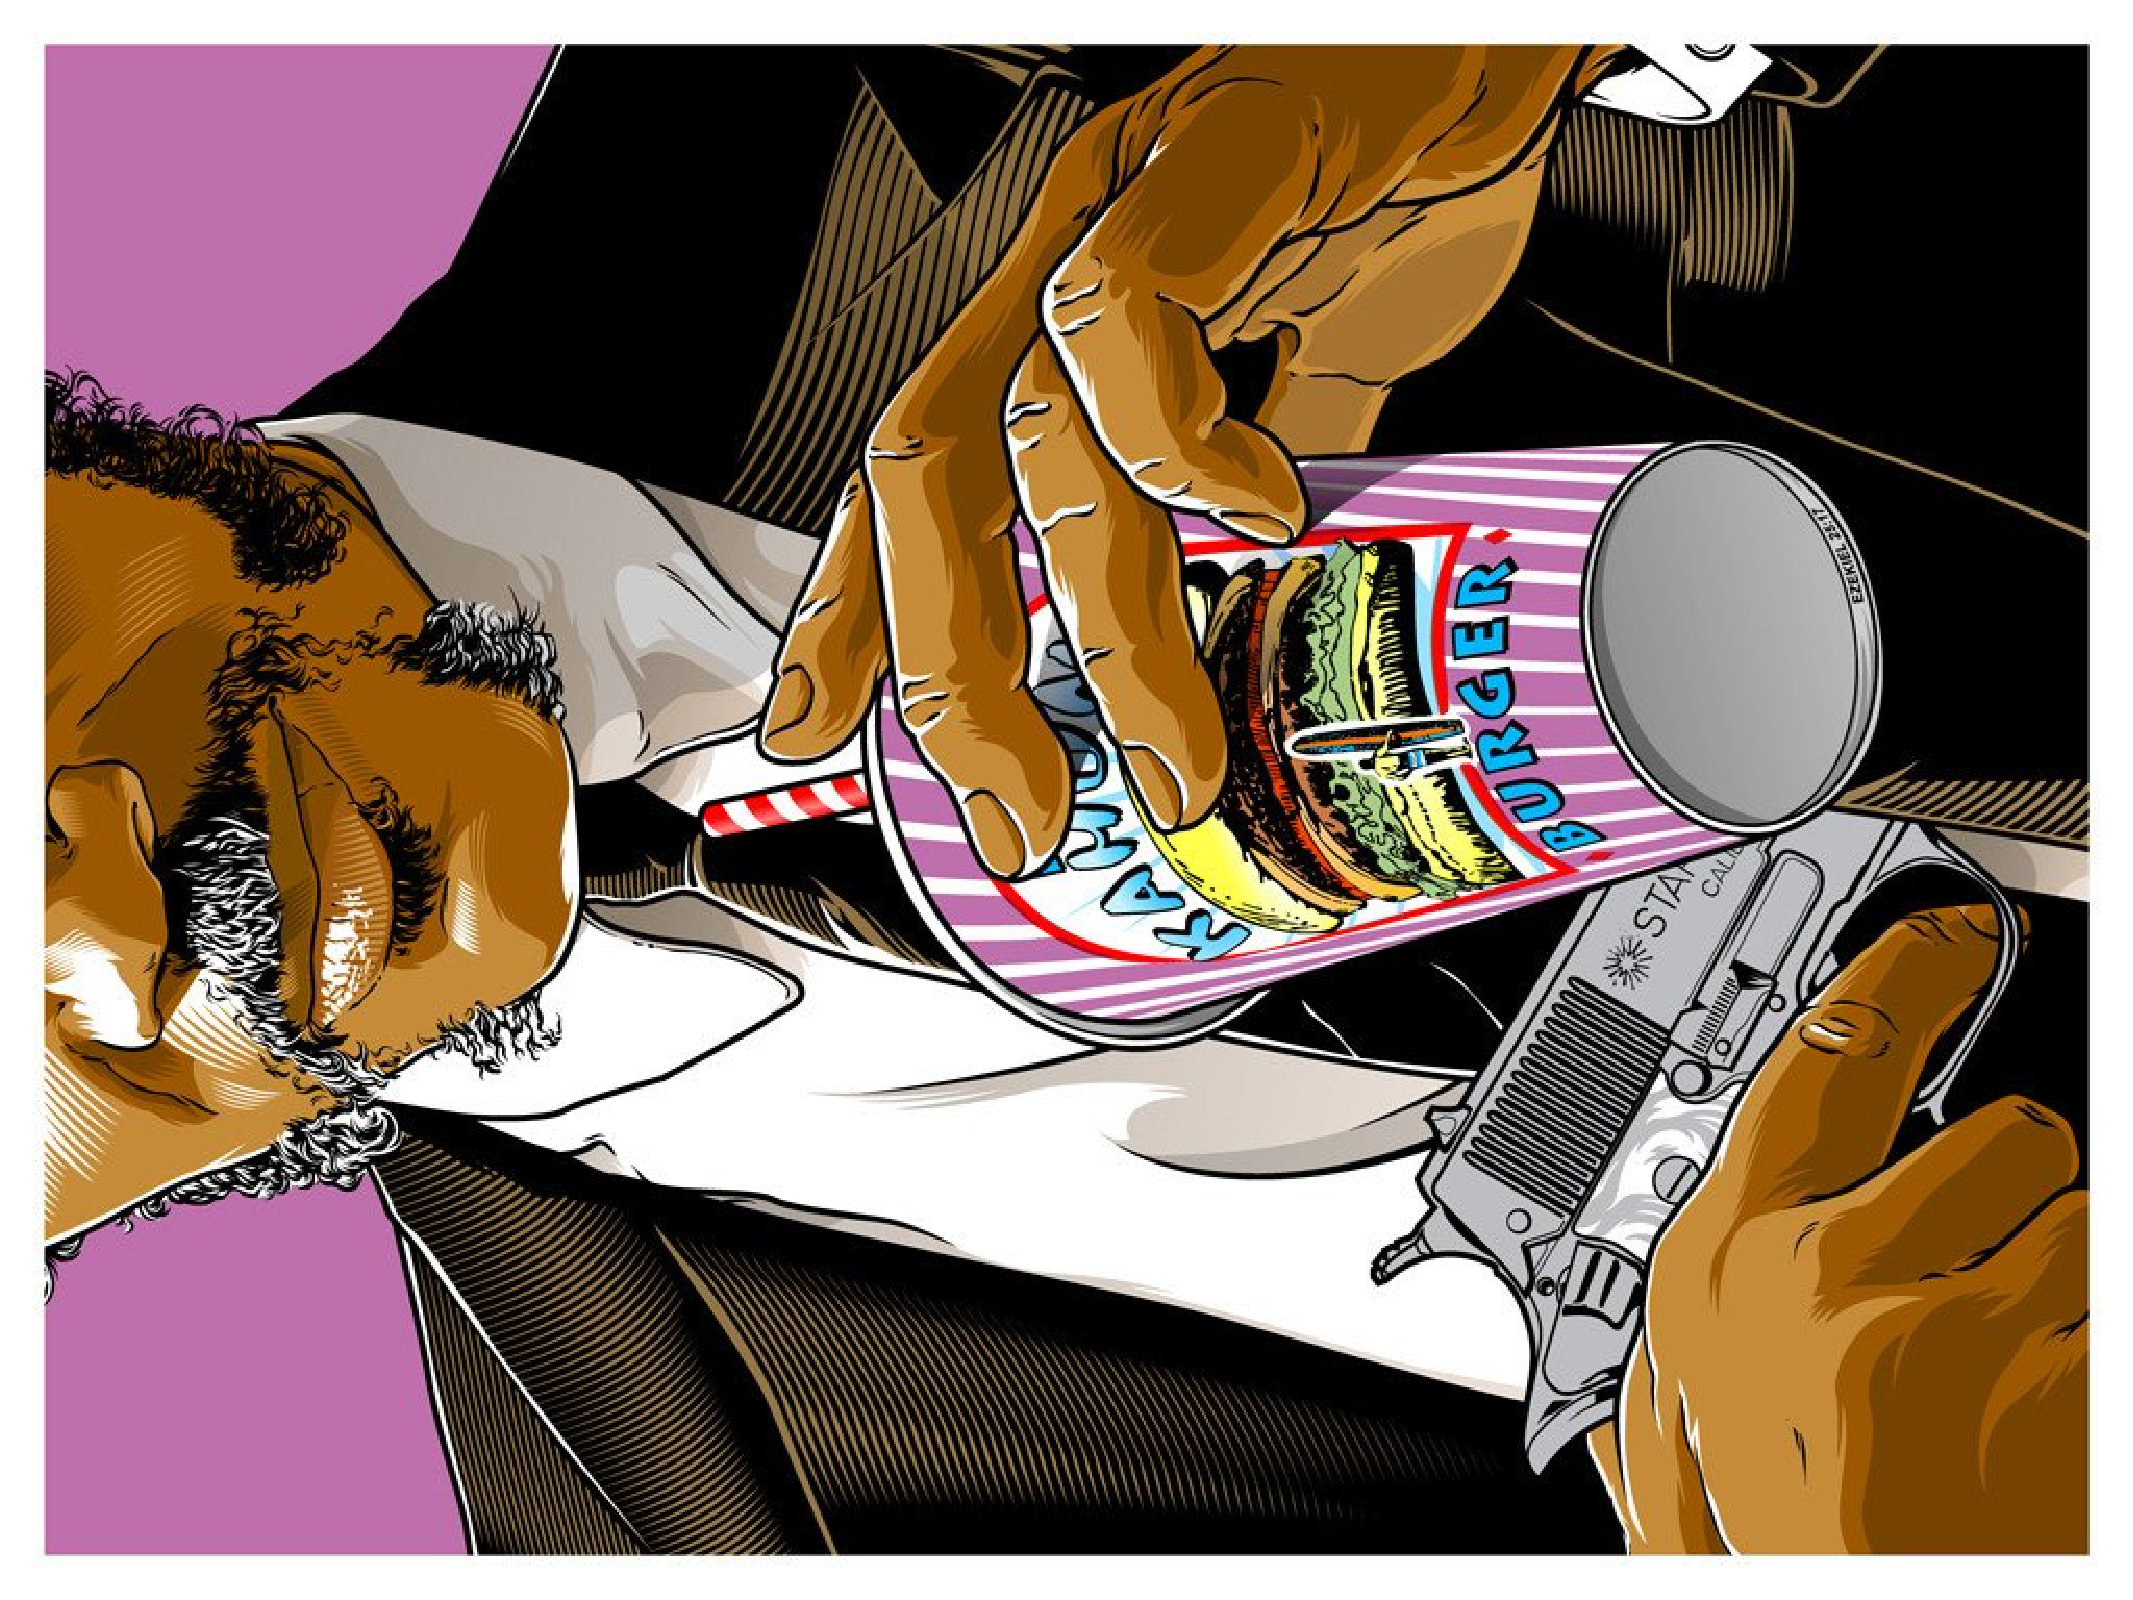
\includegraphics[width=0.82\linewidth, angle=270, scale=1.3]{pop1.pdf}
\end{minipage}
\hfill
\begin{minipage}[h!]{0.3\linewidth} 

\includegraphics[width=0.8\linewidth, height=0.21\textheight]{pop3.pdf}
\end{minipage}
\hfill
\begin{minipage}[h!]{0.3\linewidth} 
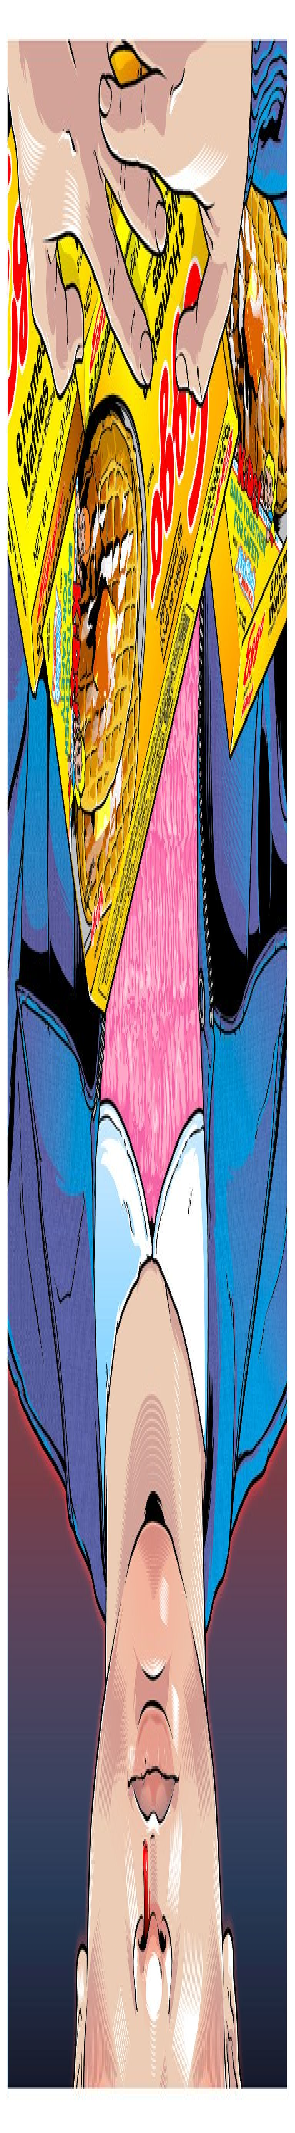
\includegraphics[width=0.8\linewidth, height=0.21\textheight, angle=180]{pop2.pdf}
\end{minipage}
\vfill
\begin{minipage}[h!]{0.3\linewidth} 
\includegraphics[width=0.8\linewidth]{pop5.pdf}
\end{minipage}
\hfill
\begin{minipage}[h!]{0.3\linewidth} 
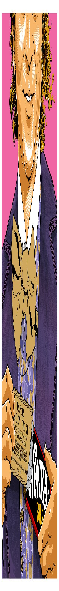
\includegraphics[width=0.8\linewidth, height=0.21\textheight]{pop7.pdf}
\end{minipage}
\hfill
\begin{minipage}[h!]{0.3\linewidth} 
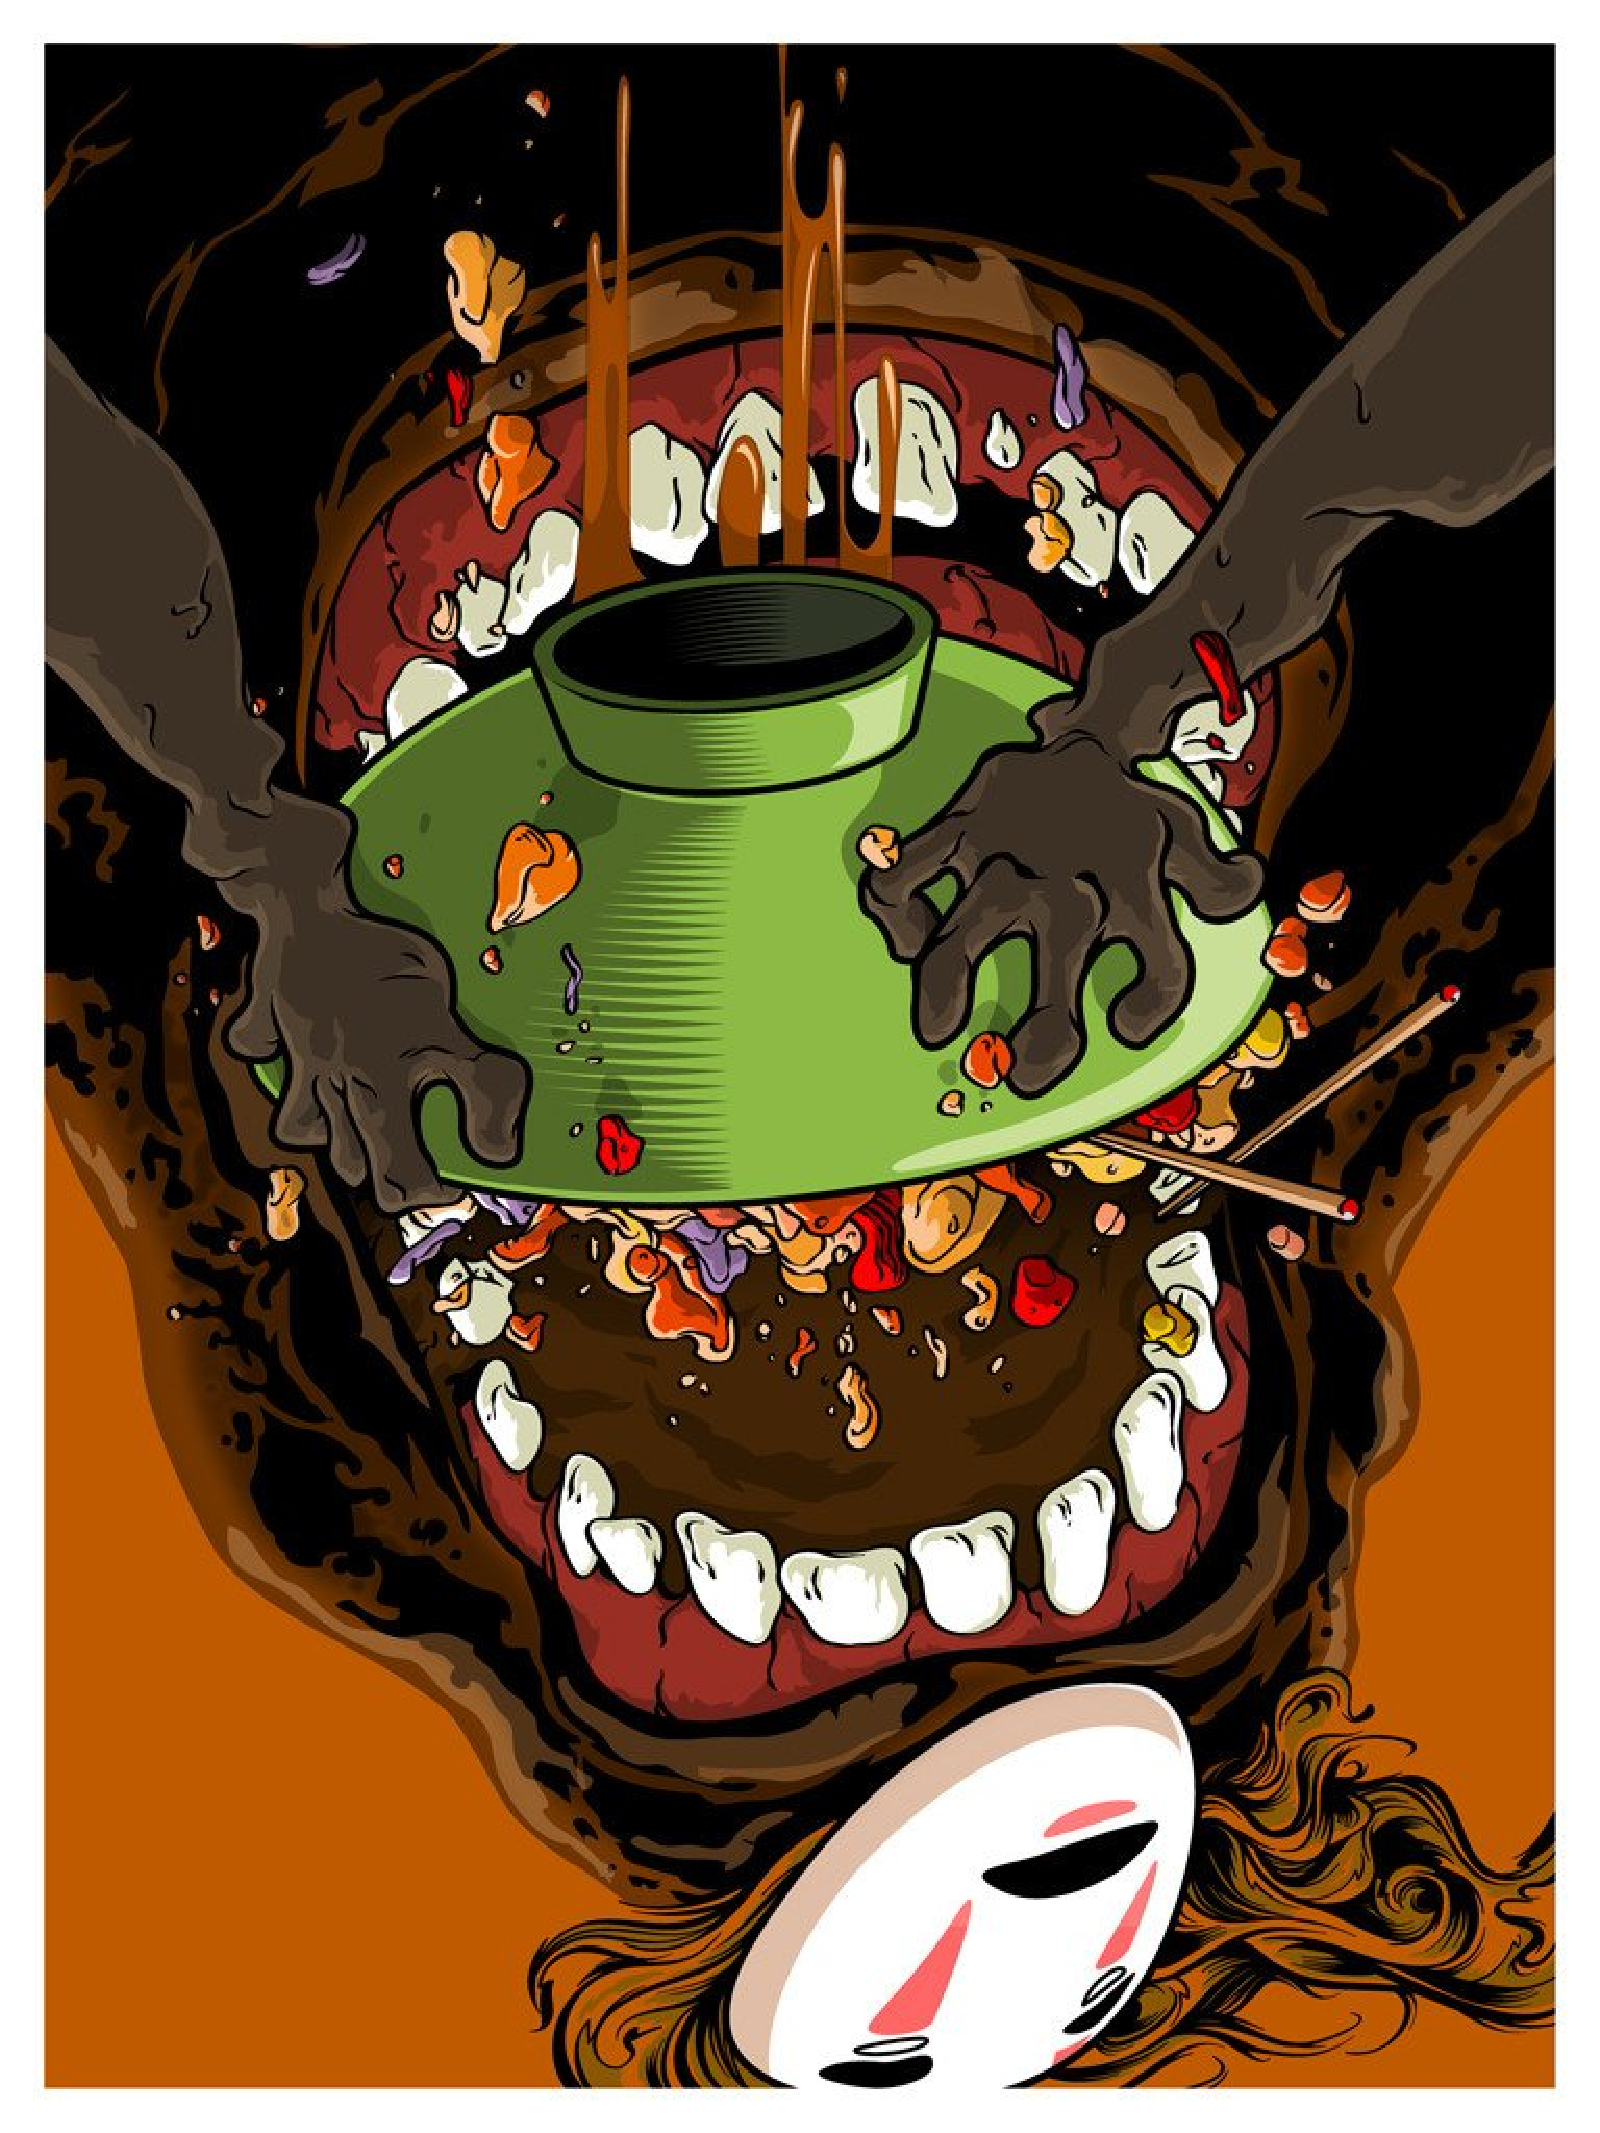
\includegraphics[width=0.8\linewidth, angle=180]{pop6.pdf}
\end{minipage}
\caption{Это что поп арт?}
\end{figure}
\end{document}